\chapter{Annexes / Divers}
\section{Quelques fonctions sur les listes}
 
\begin{footnotesize}
\begin{tabular}{l|l} \hline
\textsc{Scheme} & \textsc{Ocaml} \\ \hline
\begin{minipage}{2.8in}
\begin{Verbatim}

(define (somme l)
 (if (null? l)
   0
   (+ (car l) (somme (cdr l)))))
   
\end{Verbatim}
\end{minipage}
&
\begin{minipage}{2.8in}
\begin{Verbatim}

let rec somme l =
  match l with
  | [] -> 0
  | hd::tl -> hd + somme(tl)  
  
\end{Verbatim} 
\end{minipage} \\ \hline
\begin{minipage}{2.8in}

\begin{Verbatim}

f car (f car (... (f car acc)...))

(define (foldright f acc l)
 (if (null? l)
  acc
  (f (car l) (foldright f acc (cdr l)))))
\end{Verbatim}
\end{minipage}
&
\begin{minipage}{2.8in}

\begin{Verbatim}

f hd (f hd (... (f hd acc)...))

let rec foldright f acc l =
  match l with
  | [] -> acc
  | hd::tl -> f hd (foldright f acc tl)
  
\end{Verbatim}
\end{minipage} \\ \hline
\begin{minipage}{2.8in}
\begin{Verbatim}

f (... (f (f acc car) car)...) car)

(define (foldleft f acc l)
 (if (null? l)
  acc
  (foldleft f (f (car l) acc) (cdr l))))
  
\end{Verbatim}
\end{minipage}
&
\begin{minipage}{2.8in}
\begin{Verbatim}

f (... (f (f acc hd) hd)...) hd)

let rec foldleft f acc l =
  match l with
  | [] -> acc
  | hd::tl -> foldleft f (f acc hd) tl
  
\end{Verbatim}
\end{minipage} \\ \hline
\begin{minipage}{2.8in}
\begin{Verbatim}

(foldleft * 1 '(1 2 3 4))
-> 24

\end{Verbatim}
\end{minipage}
&
\begin{minipage}{3.0in}
\begin{Verbatim}

# foldleft ( * ) 1 [1;2;3;4] ;;
- : int = 24

\end{Verbatim}
\end{minipage} 

\end{tabular}

\end{footnotesize}
\section{Les listes mutables}

En \textsc{Scheme}, nous avons les fonctions \verb+set-car!+ et \verb+set-cdr!+ qui nous permettent de modifier physiquement
 le car et le cdr d'un doublet.
Nous pouvons par exemple définir la liste circulaire \verb+(a b c a b c ...)+
\begin{Verbatim}
(define maliste (list 'a 'b 'c))
(set-cdr! (cddr maliste) maliste)
 maliste
 -> #0= (a b c . #0#)
\end{Verbatim}
L'affichage de la liste infine provient de l'interprète DrRacket.


Essayons de reproduire cela en \textsc{Ocaml}
(de manière intuitive et sûrement très maladroite\ldots)
\begin{Verbatim}

exception Listenulle
type liste = Nil | Cons of int ref * liste ref ;;

let set_car d v =
	match d with
	| Nil -> raise Listenulle
	| Cons(car,cdr) -> car:=v  ;;
	
let set_cdr d v =
	match d with
	| Nil -> raise Listenulle
	| Cons(car,cdr) -> cdr:=v ;;
	
let  cdr l =
 match l with
 | Nil -> raise Listenulle
 | Cons(tete, reste) when !reste <> Nil -> reste

let maliste = Cons(ref 1 , ref ( Cons (ref 2, ref ( Cons (ref 3, ref Nil))) ))
set_cdr (!cdr !(cdr maliste)) maliste ;;

# maliste;;
- : liste =
Cons ({contents = 1},
 {contents =
   Cons ({contents = 2},
    {contents =
      Cons ({contents = 3},
       {contents =
         Cons ({contents = 1},
          {contents =
            Cons ({contents = 2},
             {contents =
               Cons ({contents = 3},
               	...
               	
\end{Verbatim}

\section{Les listes infinies ou \textit{streams}}	
Les \textit{streams} sont des listes infinies.

Pour pouvoir les représenter, nous utilisons le fait que le corps d'une lambda n'est pas évalué, 
comme nous l'avons vu en $\lambda$-calcul avec la
stratégie de la $\beta$-réduction faible.


Une lambda \verb+fun()->2*2+\ \imp\ \verb+- : unit -> int = <fun>+ est en fait considérée 
comme une \textit{valeur}. Seul son appel provoquera l'évaluation de la lambda
\verb+(fun() -> 2*2) ()+\ \imp\  \verb+- : int = 4+

Un \textit{stream} sera ainsi représenté comme une liste, mais dont le \verb+cdr+ ne pointera plus directement 
sur une liste, mais sera une fonction dont le corps sera la liste. L'évaluation du \verb+cdr+ est ainsi retardé.
 
\begin{Verbatim}
type 'a stream = Cons of 'a * (unit -> 'a stream) ;;
let hd (Cons (h, _)) = h ;;
let tl (Cons (_, tf)) = tf () ;;

let rec from n = Cons (n, fun () -> from (n+1));;
let entiers = from 0 ;;
let rec take n s =
  if n=0 then []
  else hd s :: take (n-1) (tl s) ;;

# take 30 entiers
- : int list =
[0; 1; 2; 3; 4; 5; 6; 7; 8; 9; 10; 11; 12; 13; 14; 15; 16; 17; 18; 19; 20;
 21; 22; 23; 24; 25; 26; 27; 28; 29]
\end{Verbatim}

Nous pouvons aussi modéliser la fraction continue représentant $\sqrt{2}$ :
\begin{equation*}
\sqrt{2} = 1 + \cfrac{1}{2
+ \cfrac{1}{2
+ \cfrac{1}{\ddots
 } } }
\end{equation*}
Voici le code \textsc{Ocaml}. Je n'ai pas trouvé de manière plus élégante pour exprimer le stream.
\begin{Verbatim}
let rec square2 iter =
  if (iter = 1) then 1.
  else
  1. +. ( 1. /. ( 1. +. square2 (iter - 1)))

let rec racine2cons n = Cons(square2 n, fun () -> racine2cons (n+1))

let rec racine2stream = racine2cons 1
  in take 10 racine2stream ;;

- : float list =
[1.; 1.5; 1.4; 1.41666666666666674; 1.4137931034482758; 1.41428571428571437;
 1.41420118343195256; 1.41421568627450989; 1.41421319796954315;
 1.41421362489486957]
\end{Verbatim}
Nous voyons la convergence très rapide de la fraction continue.

Cependant, le calcul \textsc{Ocaml} est très inefficace, car chaque nouvel élément de la liste recalcule la totalité de la fraction continue
en passant par la fonction \verb+square2 iter+. Si nous essayons par exemple de calculer les $10000$ premiers éléments du stream, cela prend sur ma machine une
dizaine de seconde. 

En utilisant le module \verb+Lazy+ d'\textsc{Ocaml}, nous pouvons utiliser le mécanisme
 de \textit{mémoisation}. Les valeurs du stream ne seront pas recalculées au 
2ème appel.
\begin{Verbatim}
open Lazy ;;
let racine2_10000 = take 10000 racine2stream  (* environ 10 secondes à chaque appel *)

let racine2_10000_lazy = lazy (take 10000 racine2stream) ;;
let racine2_force = force racine2_10000_lazy ;; (* uniquement long au 1er appel *)
\end{Verbatim} 



\section{Le module Graphics d'\textsc{Ocaml}, les fractales}

Nous allons ici présenter tres brievement le module Graphics.
Je reprends le code de Xavier Leroy tiré de son livre \textit{le langage \textsc{Caml}} \cite{caml}.

\begin{Verbatim}
open Graphics ;;

Graphics.open_graph "";;
Graphics.set_window_title "THE WINDOW" ;;

type  etat = { mutable x : float; mutable y : float; 
               mutable visee : float; mutable levee : bool };;
let crayon = { x = 0.0; y = 0.0; visee = 0.0; levee = false };; 
let fixe_crayon b = crayon.levee <- b;;

let pi_sur_180 =let pi = 4.0 *. (atan 1.0) in pi /. 180.0 


let tourne angle = crayon.visee <- (crayon.visee +. angle *. pi_sur_180) ;;

let zero_x = float_of_int ((size_x ()) / 2);;
let zero_y = float_of_int ((size_y ()) / 2);;

let vide_ecran () =
	set_color white;
	fill_rect 0 0 (size_x ()) (size_y ());
	set_color black;
	crayon.x <- zero_x;
	crayon.y <- zero_y;
	crayon.visee <- 0.0;
	crayon.levee <- false;
	moveto (round crayon.x) (round crayon.y);;


let avance d =
	let dx = d *. cos (crayon.visee)
	and dy = d *. sin (crayon.visee) in
	crayon.x <- crayon.x +. dx;
	crayon.y <- crayon.y +. dy;
	if crayon.levee then moveto (round crayon.x) (round crayon.y)
	else lineto (round crayon.x) (round crayon.y);;

let rec motif n c =
	if n = 0 then avance c
	else
		begin
			motif (n -1) (c /. 3.0);
			tourne 60.0;
			motif (n -1) (c /. 3.0);
			tourne (-120.0);
			motif (n -1) (c /. 3.0);
			tourne 60.0;
			motif (n -1) (c /. 3.0)
		end;;

let flocon n c =
  for i = 1 to 3 
   do 
     motif n c; tourne (-120.0)
   done;;

  flocon 1 100.0;		flocon 2 100.0;	  flocon 3 100.0;  flocon 4 100.0;	
\end{Verbatim}

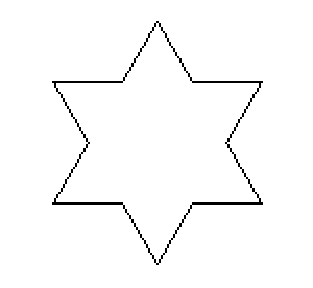
\includegraphics[width=3.5cm, height=3cm]{flocon1.pdf}
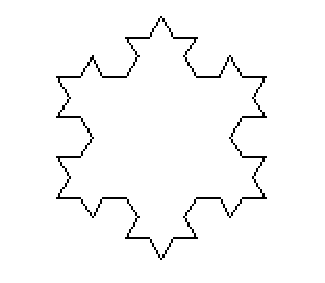
\includegraphics[width=3.5cm, height=3cm]{flocon2.pdf}
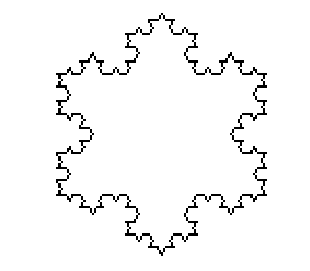
\includegraphics[width=3.5cm, height=3cm]{flocon3.pdf}
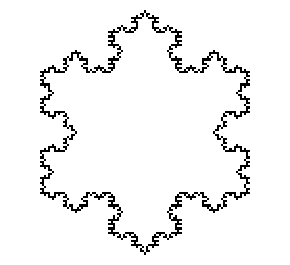
\includegraphics[width=3.5cm, height=3cm]{flocon4.pdf}


\begin{figure}[H]
	\centering
	\caption{Les côtes de la Bretagne}
	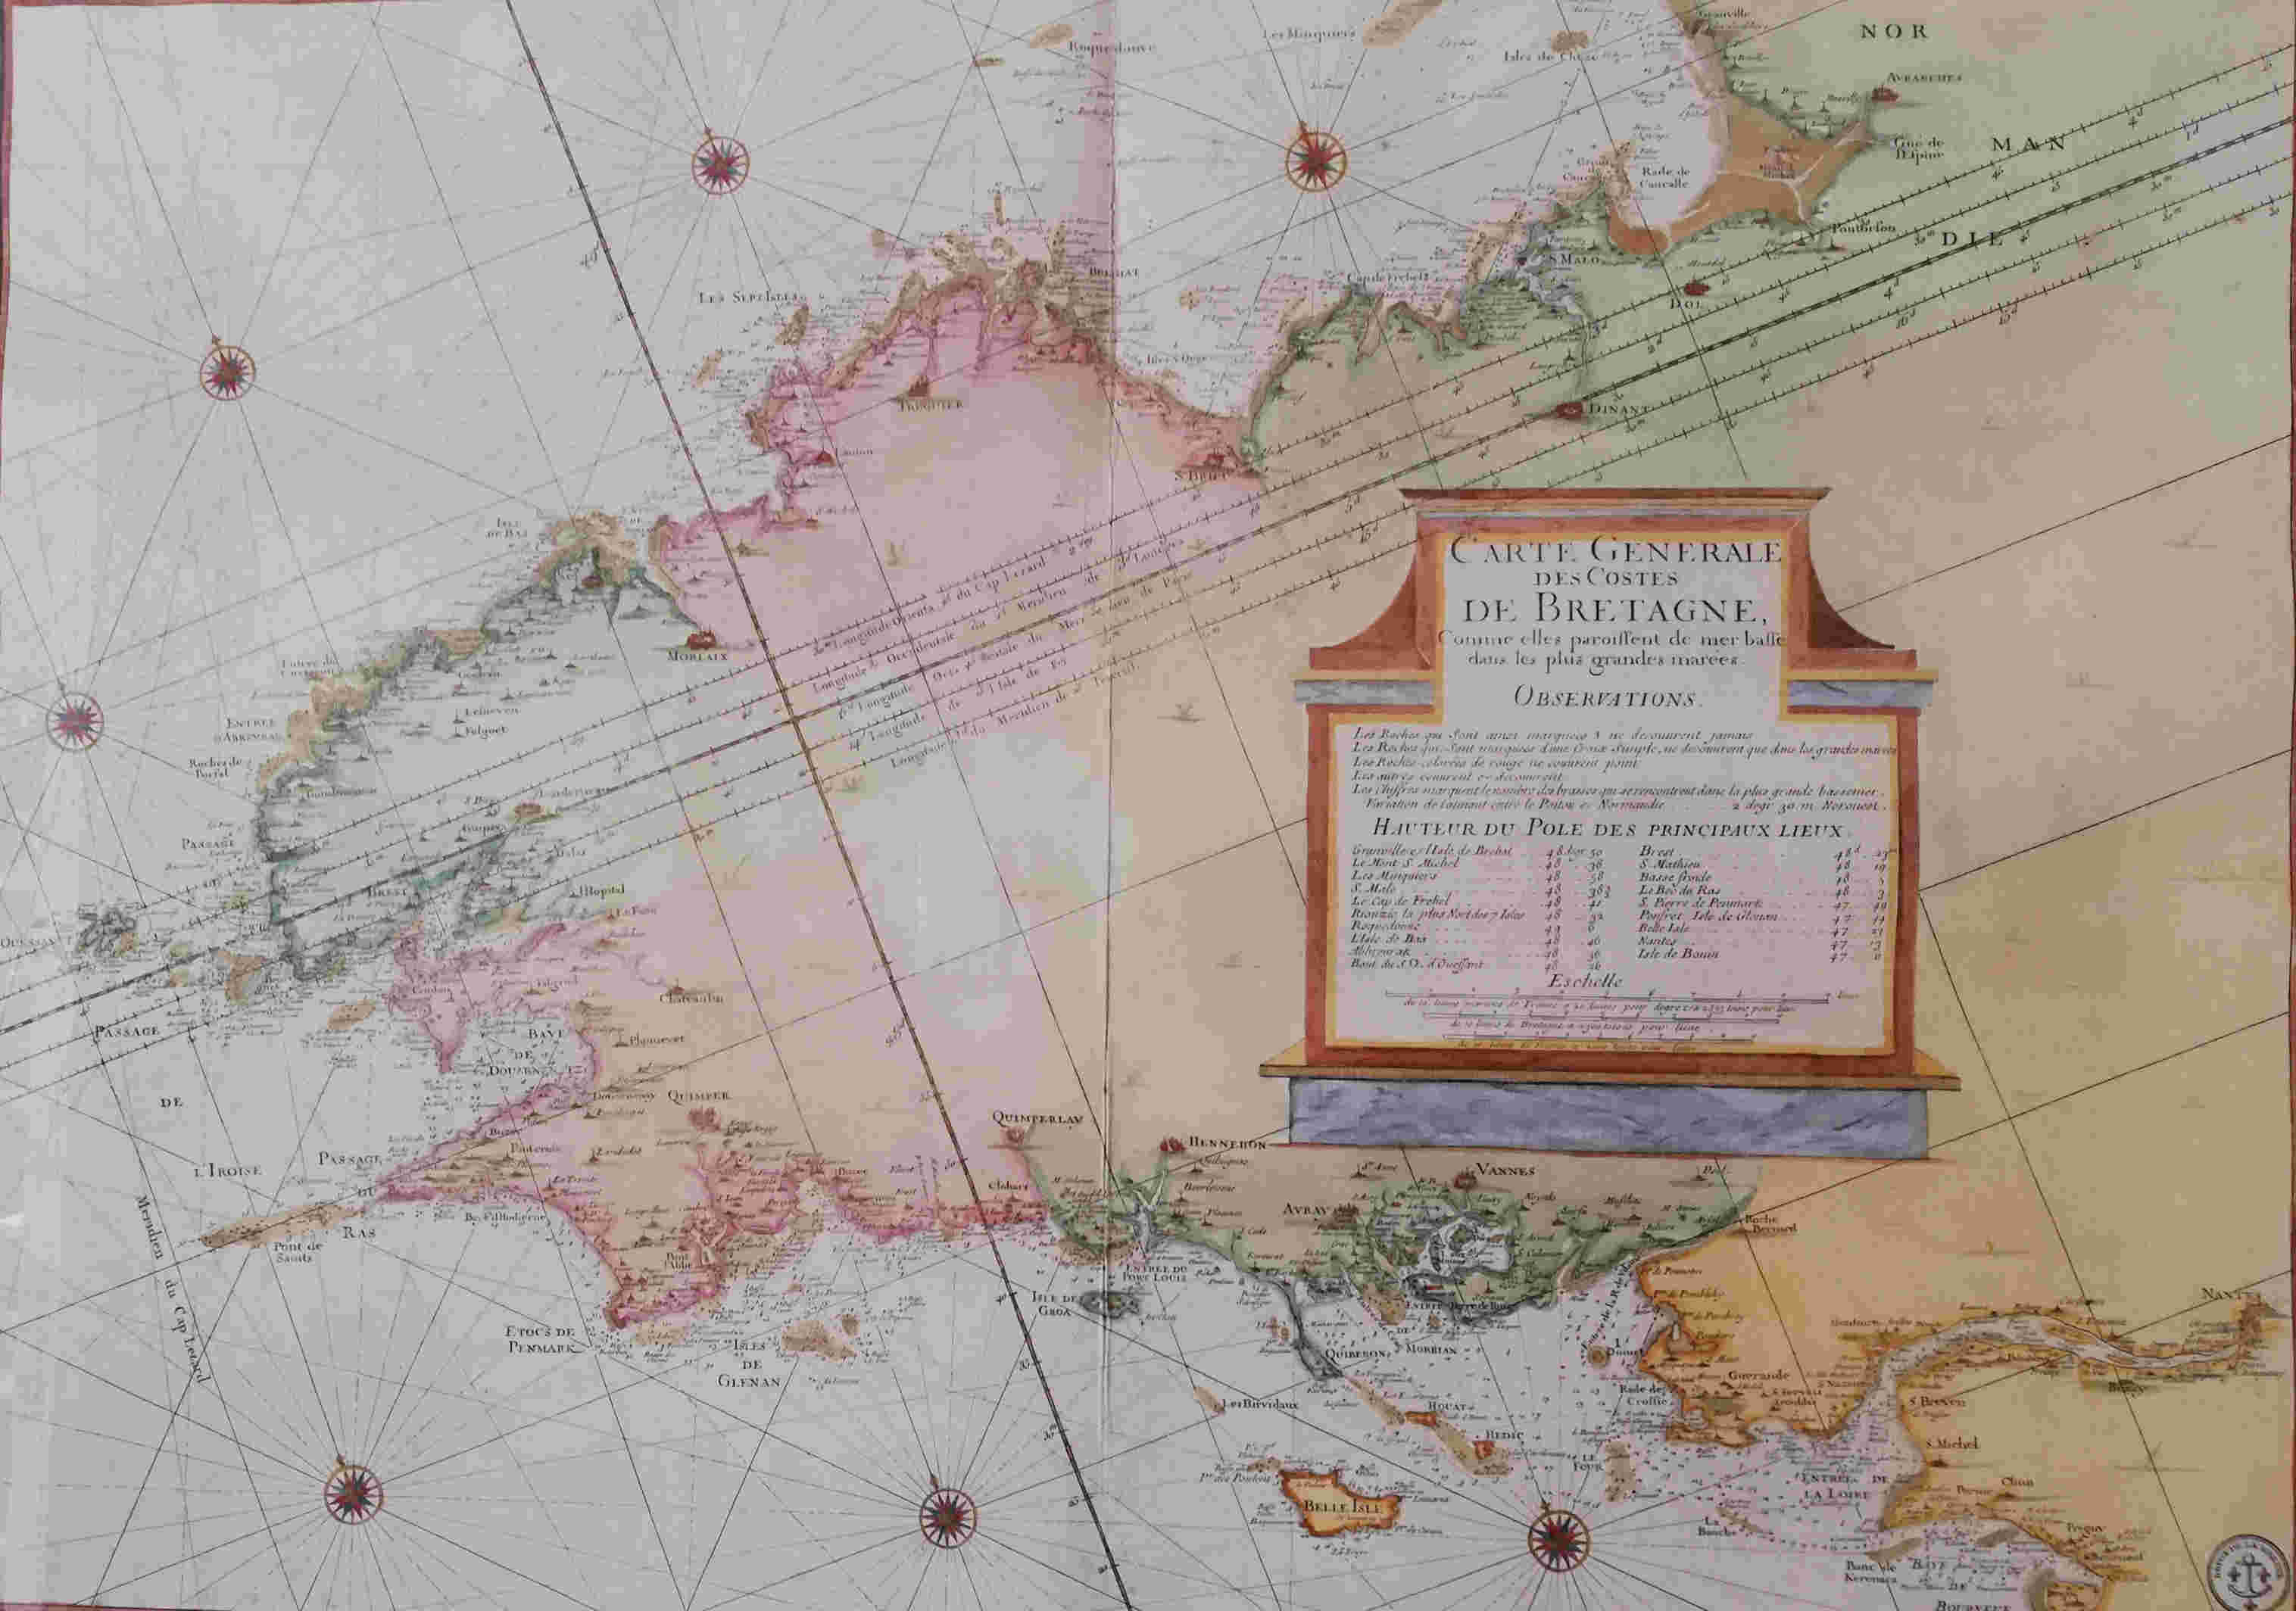
\includegraphics[width=4.0cm]{bretagne3.jpg}
\end{figure}

Les objets fractales ont une propriété surprenante : ils ont une aire finie, mais un périmètre infini.
A l'itération $n$, le périmètre de notre flocon est de $3.(\frac{4}{3})^n$. Et nous avons bien entendu 
$\lim_{n \rightarrow \infty} 3.(\frac{4}{3})^n =\infty $


La longueur des côtes de la Bretagne est-elle aussi infinie ?
\textit{L'Atlantique ronge nos côtes.} \cite{vh}

\subsubsection{L'ensemble de Mandelbrot}
l'ensemble de Mandelbrot est une fractale définie comme l'ensemble des points $c$ 
du plan complexe pour lesquels la suite des nombres complexes définie comme ci-dessous est 
\textbf{bornée}.

$$
\begin{cases}
	z_0=0\\
	z_{n+1}=z_n^2+c
\end{cases}
$$
Voir le bon article \url{https://fr.wikipedia.org/wiki/Ensemble_de_Mandelbrot}

On montre que si la suite des modules des $z_n$ est strictement supérieure à 2 pour un certain indice alors,
cette suite est croissante à partir de cet indice, et elle tend vers l'infini.
Donc notre test d'appartenance à l'ensemble s'arrêtera au-delà de la valeur 2.

Pour estimer la convergence, nous nous arrêterons à la valeur $z_{300}$.
Nous utilisons également l'hypothèse que l'ensemble de Mandelbrot se situe dans le plan complexe
$(-2.00:0.50), (-1.25:1.25)$
\begin{Verbatim}
open Complex ;;   (* {re=2.; im=4.} *)

let appartient c =
	let rec loop n z =
		if (n > 300) then true
		else if ((norm2 z) > 4.) then false
					else loop (n+1) (add c (mul z z)) 
	in loop 0 c  

#load "/home/vincent/.opam/ocaml-base-compiler/lib/graphics/graphics.cma" ;;
#require "graphics" ;; 
open Graphics ;;
Graphics.open_graph " 500x200+0-0" ;;
Graphics.set_window_title "Mandelbrot" ;;
Graphics.set_color Graphics.blue;;

let mandelbrot () =
	for i = (-200) to 50
		do
		  for j=(-125) to 125
			do
			  if (appartient {re=((float_of_int i)/.100.); im=((float_of_int j)/.100.)}) 
			  then plot (200+i) (200+j) 
			done
		done 
\end{Verbatim}

\begin{figure}[H]
	\centering
	\caption{L'ensemble de Mandelbrot}
	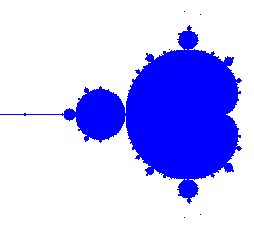
\includegraphics[width=4.0cm]{mandelbrot.png}
\end{figure}

\section{Utilisation de \MF}
\MF\ est un langage créé par D. Knuth \cite{mf}. Il permet le
design de nouvelles fontes de manière très élégante sous forme d'équations.
La programmation se fait principalement de manière déclarative.

Je me suis  amusé ici à créer le symbole  \imp que j'ai souvent
utilisé dans cet article, principalement dans la section sur le $\lambda$-calcul. 

\begin{figure}[H]
	\centering
	\caption{\imp}
	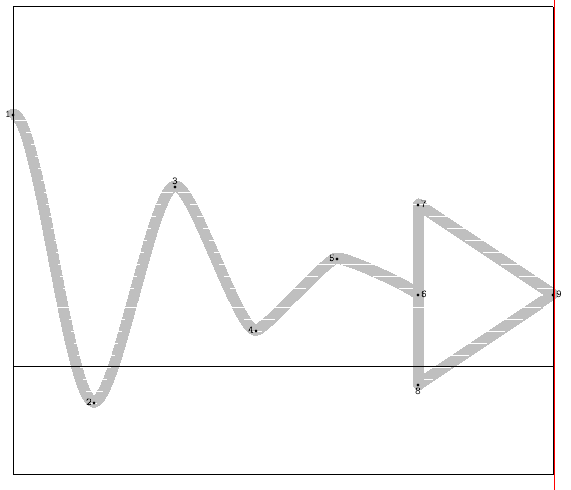
\includegraphics[width=4.0cm]{imp.png}
\end{figure}
Voici le bout de code qui a permis de définir ce symbole:
\begin{Verbatim}
%file name: beta.mf

beginchar("D",15pt#,10pt#,3pt#);
% proportion ligne vs triangle 3/4 1/4
prop:=3/4;

y1=h-d; y2=1/5h-d; y3=4/5h-d; 
y4=2/5h-d; y5=3/5h-d; y6=1/2h-d;  
y7=3/4h-d; y8=1/4h-d; y9=h/2-d;

x1=0; x2=1/5*prop*w; x3=2/5*prop*w;
x4=3/5*prop*w; x5=4/5*prop*w; x6=prop*w;
x7=x8=x6; x9=w;

pickup pencircle scaled 0.3pt;
draw z1{right}..tension 6..z2{right}..tension 5..z3{right}
     ..tension 4..z4{right}..tension 4..z5{right}..tension 3..z6;
draw z7--z8--z9--cycle; 
labels(range 1 thru 9);
endchar;
end
\end{Verbatim}

Nous avons également représenté notre fractale \snow avec le langage \MF .
Cela s'écrit très facilement, car le langage de Knuth permet l'utilisation
de macros récursives.

\begin{Verbatim}
%file name: snow.mf
%mode_setup;
%shape for the character S

i:=1;

def dessine(expr debut, fin) =
z[i]=debut;
z[i+1]=1/3[debut, fin];
z[i+2]= (z[i+1]-z[i]) rotated 60 shifted z[i+1];
z[i+3] = 2/3[debut, fin] ;
z[i+4] = fin ;  
pickup pencircle scaled 0.1pt;
draw z[i]--z[i+1]--z[i+2]--z[i+3]--z[i+4];
i:=i+5;
enddef;

def motif (expr debut, fin, n) =
if (n=1):dessine(debut,fin) else: 
	motif(debut, 1/3[debut,fin], n-1) ;
	motif(1/3[debut,fin],
		(1/3[debut,fin] - debut) rotated 60 shifted (1/3[debut,fin]), n-1) ;
	motif((1/3[debut,fin] - debut) rotated 60 shifted (1/3[debut,fin]),
		(1/3[debut,fin] -debut) shifted (1/3[debut,fin]), n-1) ;
	motif((1/3[debut,fin] - debut) shifted (1/3[debut,fin]), fin, n-1) ;
fi;
enddef;

beginchar("S",15pt#,15pt#,5pt#); "The snowflake" ;
motif((0,0), (w/2,h),4);
motif((w/2,h), (w,0),4);
motif((w,0), (0,0),4);
endchar;
end
\end{Verbatim}

Voici le résultat:
\begin{figure}[H]
	\centering
	\caption{\snow}
	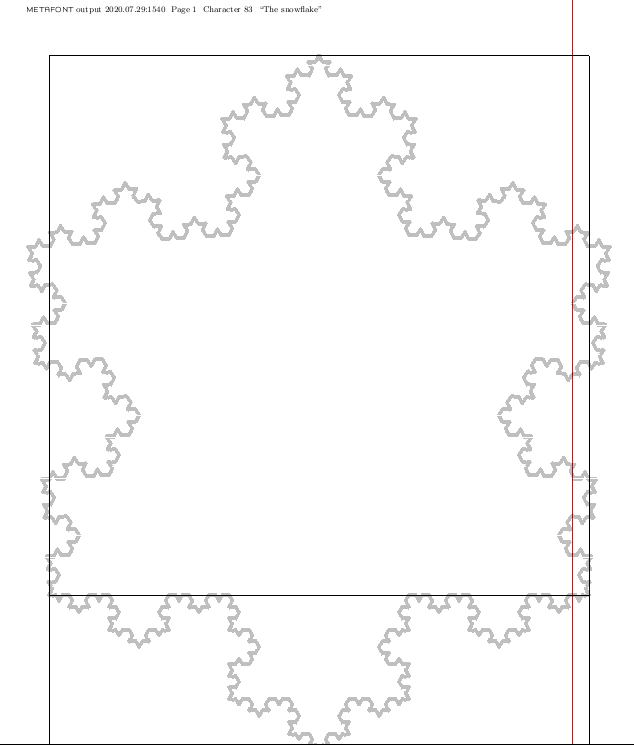
\includegraphics[width=4.0cm]{snow.png}
\end{figure}

\section{The boxes}
Nous avons vu comment représenter un environnement comme une liste
d'associations avec des paires \verb+variable.valeur+.
Une autre méthode est d'utiliser le principe de \textit{box} qui encapsule la
valeur dans une lambda. La \textit{box} est une lambda qui prend une valeur à  sa
création. Puis elle réagit à  deux messages qui permettent respectivement
d'afficher la valeur capturée ou de la modifier avec la procédure \verb+set!+


Voici l'implémentation en Scheme:
\begin{Verbatim}
(define (box value)
  (lambda (msg)
    (case msg
      ("get" value)
      ("set" (lambda (new-value) (set! value new-value))))))

(define (make-box value)
  (box value))

(define maboite (make-box 4))
(maboite "get")
((maboite "set") 5)
\end{Verbatim}

En \textsc{Ocaml}, nous pouvons rédiger le code ci-dessous:
\begin{Verbatim}
exception Erreur

let box value0 =
	let value = ref value0 in
	fun message ->
		match message with
		| "get" -> (fun any -> print_int !value)
		| "set" -> (fun newvalue -> (value := newvalue ; print_int !value ))
		| "reset"-> (fun any -> (value := value0 ; print_int !value))
		| _ -> raise Erreur
		
		
let maboite = box 5 ;;
(maboite "get") 0 ;;
(maboite "set") 1976 ;;
(maboite "get") 0 ;;
(maboite "reset") 0 ;;
\end{Verbatim}

\section{Les modules \textsc{Ocaml}. Modélisation d'un monoïde}
Un monoïde est une structure algébrique qui possède une loi de composition
interne associative et un élément neutre.
Représentons cette structure en \textsc{Ocaml}, en définissant un module.
Nous reprenons ici l'excellent article 
https://blog.derniercri.io/observons-une-premiere-structure-algebrique-appliquee-a-linformatique-le-monoide/
\begin{Verbatim}
module type MONOID =
sig
type t
val ( <+> ) : t -> t -> t
val neutral : t	
end

module String_monoid : MONOID with type t = string  =
struct
type t = string
let ( <+> ) = (^)
let neutral = ""
end

String_monoid.("abc" <+> "def" <+> neutral)
-> String_monoid.t = "abcdef"	
\end{Verbatim}

En algèbre, un morphisme (ou homomorphisme) est une application entre deux structures algébriques
de même espèce.

Pour les  monoïdes, un morphisme est une application 
$f:(M,*,e)\longrightarrow (M',\star ,e')$ , entre deux monoïdes $ (M,*,e)$ et 
$(M',\star , e')$ qui vérifie :
\begin{itemize}
	\item $\forall (g,h)\in M^{2},~f(g*h)=f(g)\star f(h)$
	\item $f(e)=e'$
\end{itemize}
\begin{Verbatim}
#load "Str.cma"

let count  t =  split (regexp " ") t   |> List.length ;;

let pageA = "Hello World "
let pageB = "Foo bar "
let pageC = "O Caml " ;;

count String_monoid.(pageA <+> pageB <+>  pageC) ;;
count(String_monoid.(pageA)) + count(String_monoid.(pageB)) + count(String_monoid.(pageC));;
\end{Verbatim}
Nous avons ici utilisé l'opérateur \verb+|>+ défini comme suit \verb+let ( |> ) x f = f x+

Cette fonction \verb+count+ est ainsi un morphisme entre le monoïde \verb+String_monoid+ et 
le monoïde des entiers (avec $+$ comme fonction de composition interne et $0$
comme élément neutre)
\section{Machine Learning and Neural Networks}

\subsection{Introduction}

Nous implémentons en R un réseau de neurones réduit à sa plus simple expression.
Il n'aura que deux couches de neurones.
Le langage R est ici commode pour ses opérations natives sur les matrices.
Nous pourrons voir ensuite comme transposer ce code en \textsc{Ocaml}.

Nous entraînerons notre NN sur la base du jeu de test MNIST.
Le  "training set" contient 60000 exemples, et le "test set" 10000 exemples.
Nous pourrons nous documenter plus précisément avec l'excellent ouvrage de François Chollet \cite{deepR}.

\subsection{Un peu de théorie}

Soit les 150 observations suivantes représentées par la matrice $X_{150,784}$ (ou tensor 2 dimensions) comprenant 150 lignes pour les 150 observations et 784 colonnes pour les 784 features des observations.

2 matrices de poids $W^1_{32,150}$ et $W^2_{10,150}$ sont utilisées.

\begin{itemize}
	\item 1er layer de 32 neurones
	\item 2nd layer de 10 neurones
\end{itemize}

La sortie $OUTPUT_{150,10}$ est une matrice de 150 lignes avec les 10 colonnes représentant 
les 10 features que l'on cherche à reconnaître.

Voici le schéma simplifié du NN à 2 couches:

$$
X \longrightarrow \otimes W^1 \rightarrow  Z^1 \rightarrow \sigma \rightarrow LAYER^1 \longrightarrow
\otimes W^2 
\rightarrow Z^2 
\rightarrow 
\sigma 
\rightarrow \hat{Y} 
>> LOSS(\hat{Y}, Y)
$$

\subsection{Calcul matriciel}

Cela donne le calcul matriciel ci-dessous:
\begin{footnotesize}
\begin{align*}
\begin{pmatrix}
x_{1,1} & x_{1,2} & \cdots & x_{1,784} \\
x_{2,1} & x_{2,2} & \cdots & x_{2,784} \\
\vdots  & \vdots  & \ddots & \vdots  \\
x_{150,1} & x_{150,2} & \cdots & x_{150,784} 
\end{pmatrix}
\times
\begin{pmatrix}caml
w^1_{1,1} & w^1_{1,2} & \cdots & w^1_{1,32} \\
w^1_{2,1} & w^1_{2,2} & \cdots & w^1_{2,32} \\
\vdots  & \vdots  & \ddots & \vdots  \\
w^1_{784,1} & w^1_{784,2} & \cdots & w^1_{784,32} 
\end{pmatrix}
&= 
\begin{pmatrix}
z^1_{1,1} & z^1_{1,2} & \cdots & z^1_{1,32} \\
z^1_{2,1} & z^1_{2,2} & \cdots & z^1_{2,32} \\
\vdots  & \vdots  & \ddots & \vdots  \\
z^1_{150,1} & z^1_{150,2} & \cdots & z^1_{150,32} 
\end{pmatrix}
\\
\sigma(
\begin{pmatrix}
z^1_{1,1} & z^1_{1,2} & \cdots & z^1_{1,32} \\
z^1_{2,1} & z^1_{2,2} & \cdots & z^1_{2,32} \\
\vdots  & \vdots  & \ddots & \vdots  \\
z^1_{150,1} & z^1_{150,2} & \cdots & z^1_{150,32} 
\end{pmatrix}
)
\times
\begin{pmatrix}
w^2_{1,1} & w^2_{1,2} & \cdots & w^2_{1,10} \\
w^2_{2,1} & w^2_{2,2} & \cdots & w^2_{2,n} \\
\vdots  & \vdots  & \ddots & \vdots  \\
w^2_{32,1} & w^2_{32,2} & \cdots & w^2_{32,10} 
\end{pmatrix}
&= 
\begin{pmatrix}
z^2_{1,1} & z^2_{1,2} & \cdots & z^2_{1,10} \\
z^2_{2,1} & z^2_{2,2} & \cdots & z^2_{2,10} \\
\vdots  & \vdots  & \ddots & \vdots  \\
z^2_{150,1} & z^2_{150,2} & \cdots & z^2_{150,10} 
\end{pmatrix}
\\
\sigma(
\begin{pmatrix}
z^2_{1,1} & z^2_{1,2} & \cdots & z^2_{1,10} \\
z^2_{2,1} & z^2_{2,2} & \cdots & z^2_{2,10} \\
\vdots  & \vdots  & \ddots & \vdots  \\
z^2_{150,1} & z^2_{150,2} & \cdots & z^2_{150,10}
\end{pmatrix}
)
&=
\begin{pmatrix}
\hat{y}_{1,1} & \hat{y}_{1,2} & \cdots & \hat{y}_{1,10} \\
\hat{y}_{2,1} & \hat{y}_{2,2} & \cdots & \hat{y}_{2,10} \\
\vdots  & \vdots  & \ddots & \vdots  \\
\hat{y}_{150,1} & \hat{y}_{150,2} & \cdots & \hat{y}_{150,10} 
\end{pmatrix}
\end{align*}
\begin{align*}
LOSS(Y, \hat{Y}) &= \sum (
\begin{pmatrix}
\hat{y}_{1,1} & \hat{y}_{1,2} & \cdots & \hat{y}_{1,10} \\
\hat{y}_{2,1} & \hat{y}_{2,2} & \cdots & \hat{y}_{2,10} \\
\vdots  & \vdots  & \ddots & \vdots  \\
\hat{y}_{150,1} & \hat{y}_{150,2} & \cdots & \hat{y}_{150,10} 
\end{pmatrix}
-
\begin{pmatrix}
y_{1,1} & y_{1,2} & \cdots & y_{1,10} \\
y_{2,1} & y_{2,2} & \cdots & y_{2,10} \\
\vdots  & \vdots  & \ddots & \vdots  \\
y_{150,1} & y_{150,2} & \cdots & y_{150,10} 
\end{pmatrix}
)^2
\end{align*}

\begin{align*}
Z_1 &= X.W_1 \\
LAYER_1 &= \sigma (Z_1) \\
Z_2 &= LAYER_1 * W_2 \\
\hat{Y} &= \sigma (Z_2) \\
LOSS &= (\hat{Y} -Y)^2  
\end{align*}
\end{footnotesize}

Calculons la dérivée de la fonction $LOSS$ en fonction de $W^1$

\begin{align*}
 \frac{\delta LOSS}{\delta W_1} &=\frac{\delta LOSS}{\delta \hat{Y}} . \frac{\delta \hat{Y}}{\delta Z_2}. \frac{\delta Z_2}{\delta LAYER_1 }.\frac{\delta LAYER_1}{\delta Z_1 }. \frac{\delta Z_1}{\delta W_1 } \\ 
  &= 2(\hat{Y}-Y) . \sigma ^\prime (Z_2) . W_2 . \sigma ^\prime (Z_1). X
\end{align*}

$2(\hat{Y}-Y)$ est une matrice de dimension $(150, 10)$

$\sigma ^\prime (Z_2)$ est une matrice de dimension $(150,10)$

$W_2$ est une matrice de dimension $(32,10)$

$\sigma ^\prime (Z_1)$ est une matrice de dimension $(150,32)$

$X$ est une matrice de dimension $(150,784)$

Le calcul matriciel qui sera fait est $t(X)* \{ (2(\hat{Y}-Y) . \sigma ^\prime (Z^2) * t(W^2). \sigma ^\prime (Z^1)\}$, où $*$ est le produit matriciel et $.$ le produit d'Hadamard.
Le résultat donne une matrice de dimension $(784,32)$ qui est de même dimension que $W_1$
\begin{align*}
t(150,784)* \{(150,10).(150,10)*t(32,10).(150,32))\} &= (784,150) * \{(150,10)*(10,32).(150,32)\}\\ 
&= (784,150)*(150,32) \\
&=(784,32)
\end{align*}

 
\subsection{Fonctions d'activation}

Pour la fonction d'activation, ici appelée $\sigma$, nous utiliserons pour la première couche la fonction $relu(x) = max(o,x)$

Pour la seconde couche, nous utiliserons la fonction sigmoid $f(x)= \frac{1}{1+e^{-x}}$

\begin{figure}[H]
\centering
\caption{La fonction sigmoid}
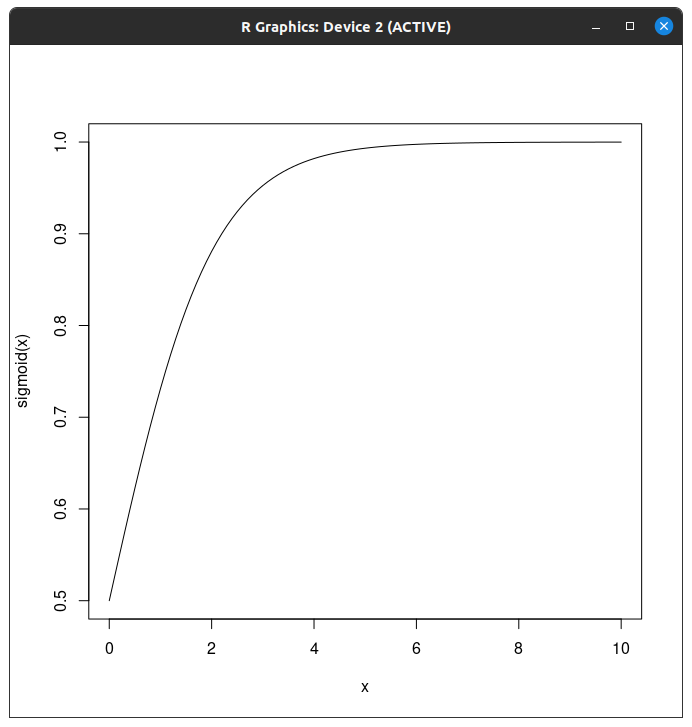
\includegraphics[width=5cm, height=5cm]{sigmoid}
\end{figure}

Voici le code en R:

\begin{Verbatim}
# the activation function
sigmoid <- function(x) {
	1.0 / (1.0 + exp(-x))
}

x=seq(0,10,0.1)
plot(x, sigmoid(x), type="l") 

# the derivative of the activation function
sigmoid_derivative <- function(x) {
	sigmoid(x) * (1.0 - sigmoid(x))
}
\end{Verbatim}


Calculons la dérivée de la fonction $LOSS$ en fonction de $W^2$ 

\begin{align}
\frac{\delta LOSS}{\delta W_2} & =\frac{\delta LOSS}{\delta \hat{Y}} . \frac{\delta \hat{Y}}{\delta Z_2}. \frac{\delta Z_2}{\delta W_2 } \\
 &= 2(\hat{Y}-Y) . \sigma ^\prime (Z_2) . LAYER_1 
\end{align}

$2(\hat{Y}-Y)$ est une matrice de dimension $(150, 10)$

$\sigma ^\prime (Z_2)$ est une matrice de dimension $(150,10)$

$LAYER_1$ est une matrice de dimension $(150,32)$

Le calcul matriciel qui sera fait est $t(LAYER_1)* (2(\hat{Y}-Y) . \sigma ^\prime (Z_2))$, où $*$ est le produit matriciel et $.$ le produit d'Hadamard.
Le résultat donne une matrice de dimension $(32,10)$ qui est de même dimension que $W_2$
$$
t(150,32) * (150,10).(150.10) = (32,150)*(150,10)=(32,10)
$$


\section{Les nombres premiers. L'algorithme RSA}

\begin{itemize}
	\item Le crible d'Erathostène (\textgreek{'Eratosjénhs}) 
	\item Leur répartition
	\item Les nombres premiers jumeaux
	\item La constante de Brun 
	\item La fonction zêta
	\item Le produit eulérien et sa convergence avec la suite harmonique
	\item Le petit théorème de Fermat
	\item La fonction \textit{indicatrice} d'Euler
	\item L'algorithme RSA
\end{itemize}

\subsubsection{Le crible}
\begin{Verbatim}
type 'a stream = Cons of 'a * (unit -> 'a stream) ;;
let hd (Cons (h, _)) = h ;;
let tl (Cons (_, tf)) = tf () ;;

let rec take n s =
	if n=0 then []
	else hd s :: take (n-1) (tl s) 

let rec entiers x = Cons(x, fun() -> entiers(x+1)) 

let rec filtre m (Cons(x,l)) =
	if x mod m = 0 then filtre m (l()) 
	else Cons(x, fun() -> (filtre m (l()))) 

let rec crible (Cons(x,l)) = Cons(x, fun()-> crible(filtre x (l())))

let premiers = crible(entiers 2) ;;
\end{Verbatim}
\begin{Verbatim}
utop # take 100 premiers ;;
- : int list =
[2; 3; 5; 7; 11; 13; 17; 19; 23; 29; 31; 37; 41; 43; 47; 53; 59; 61; 67; 71;
 73; 79; 83; 89; 97; 101; 103; 107; 109; 113; 127; 131; 137; 139; 149; 151;
 157; 163; 167; 173; 179; 181; 191; 193; 197; 199; 211; 223; 227; 229; 233;
 239; 241; 251; 257; 263; 269; 271; 277; 281; 283; 293; 307; 311; 313; 317;
 331; 337; 347; 349; 353; 359; 367; 373; 379; 383; 389; 397; 401; 409; 419;
 421; 431; 433; 439; 443; 449; 457; 461; 463; 467; 479; 487; 491; 499; 503;
 509; 521; 523; 541]
\end{Verbatim}

\subsubsection{Le produit d'Euler aka le produit eulérien}
La fonction zêta est égale au produit eulérien
\[ \zeta(s) = \sum_{n=1}^{\infty} \frac{1}{n^s} = \prod_{i=1}^\infty \frac{1}{1-p_i^{-s}} = \prod_{i=1}^\infty \frac{p_i^s}{p_i^s-1} \]

Exemple pour $s=1$ avec la suite harmonique
$$
\begin{array}{ccc}
1+ \frac{1}{2} + \frac{1}{3} + \frac{1}{4} + \frac{1}{5} +...  &=  \frac{1}{1-\frac{1}{2}} .\frac{1}{1-\frac{1}{3}}.\frac{1}{1-\frac{1}{5}}.\frac{1}{1-\frac{1}{7}}. (...) \\[\bigskipamount]
&= \frac{2.3.5.7.11.13.17.19...}{1.2.4.6.10.12.16.18...} 
\end{array}
$$

Démontrons cela
\[\zeta(1) = 1+ \frac{1}{2} + \frac{1}{3} + \frac{1}{4} + \frac{1}{5}+ \frac{1}{6}+ \frac{1}{7} +  \frac{1}{8} +... \]

Divisons par 2
\[ \frac{\zeta(1)}{2} = \frac{1}{2}+\frac{1}{4}+\frac{1}{6}+\frac{1}{8}+\frac{1}{10}+\frac{1}{12} + \frac{1}{14}+ \frac{1}{16}+... \]
 
La différence de ces 2 équations donne:
\[ \zeta(1).(1-\frac{1}{2}) = 1 + \frac{1}{3}+\frac{1}{5}+\frac{1}{7}+\frac{1}{9}+\frac{1}{11}+\frac{1}{13}+ ... \]

Divisons par 3
\[ \frac{1}{3}.(1-\frac{1}{2}).\zeta(1) = \frac{1}{3} + \frac{1}{9}+\frac{1}{15}+\frac{1}{21}+\frac{1}{27}+ \frac{1}{33}+ \frac{1}{39}+... \]

La différence donne:
\[ (1-\frac{1}{3}).(1-\frac{1}{2}).\zeta(1) = 1 + \frac{1}{5} + \frac{1}{7}+\frac{1}{11}+\frac{1}{13}+ ... \]

Divisons par 5
\[ \frac{1}{5}.(1-\frac{1}{3}).(1-\frac{1}{2}).\zeta(1) =    \frac{1}{5} + \frac{1}{25}+\frac{1}{35}+\frac{1}{55}+ ... \]

La différence donne:
\[(1-\frac{1}{5}).(1-\frac{1}{3}).(1-\frac{1}{2}).\zeta(1) = 1 + \frac{1}{7}+\frac{1}{11}+\frac{1}{13}+... \]

Nous pouvons poursuivre sur le principe du crible d'Erathostène
\[ \ldots(1-\frac{1}{5}).(1-\frac{1}{3}).(1-\frac{1}{2}).\zeta(1) = 1 \]

D'où :
$$
\begin{array}{ccc}
\zeta(1) &=& \frac{1}{(1-\frac{1}{2}).(1-\frac{1}{3}).(1-\frac{1}{5})\ldots} \\[\bigskipamount]
\zeta(1) &=& \frac{1}{\frac{1}{2}.\frac{2}{3}.\frac{4}{5}\ldots} 		\\[\bigskipamount]
\zeta(1) &=&  \frac{2.3.5.7.11.13.17.19...}{1.2.4.6.10.12.16.18...} \\[\bigskipamount]
\end{array}
$$

Le numérateur est le produit de l'ensemble des nombres premiers.
Le dénominateur est le produit de l'ensemble des nombres premiers moins 1.


Exemple pour $s=2$ avec la suite carrée
\[ 1+ \frac{1}{4} + \frac{1}{9} + \frac{1}{16} + ...  =  \frac{1}{1-\frac{1}{4}} .\frac{1}{1-\frac{1}{9}}.\frac{1}{1-\frac{1}{25}}.\frac{1}{1-\frac{1}{49}}. (...) \]



\subsubsection{Les nombres premiers jumeaux et la constante de Brun}
La somme inverse des nombres premiers jumeaux. Il y en aurait une infinité. Cependant, cette somme
 converge vers la constante de Brun.



\begin{align*}
   Brun &= (\frac{1}{3} + \frac{1}{5}) + (\frac{1}{5} + \frac{1}{7}) + (\frac{1}{11} + \frac{1}{13}) + (\frac{1}{17} + \frac{1}{19}) + (\frac{1}{29} + \frac{1}{31}) +\  ...  \\
   Brun &\approx 1,90216
\end{align*}


\begin{Verbatim}
let rec filtre_jumeaux = function
 | Cons(x,l) -> if (hd (l()) = (x+2)) then 
                  Cons(x, fun() -> Cons ((hd (l())) , (fun() ->  (filtre_jumeaux  (l())))))
                else filtre_jumeaux (l()) ;;

take 100 (filtre_jumeaux premiers) ;;

let rec inverse (Cons(x,l)) = Cons(1. /. float_of_int x, fun() -> inverse(l())) ;;

let inverse_jumeaux = inverse (filtre_jumeaux premiers) ;;

let rec somme n s =
if n=0 then 0.
else hd s +. somme (n-1) (tl s) ;;

somme 10000 inverse_jumeaux ;;
 \end{Verbatim}

 Avec les 10000 premières paires, nous sommes encore loin de $1,90216$\dots

\subsubsection{Le petit théorème de Fermat}
Si $p$ est premier et si $a$ n’est pas un multiple de $p$, alors $a^{p−1}≡1  \mod p$

\subsubsection{Le théorème d'Euler}
L'indicatrice d'Euler est une fonction, qui à tout entier naturel $n$ non nul associe
 le nombre d'entiers compris entre 1 et $n$ et premiers avec $n$. Cette fonction est nommée en anglais
 \textit{Euler's totient function}
$$
\begin{array}{ccccl}
  \varphi & : & \mathbb{N}^* & \longrightarrow & \mathbb{N}^* \\
   & & n& \longmapsto &\mathrm{card}\{ m \in \mathbb{N}^* ~|~m\le n~  \text{et}~m~\mathrm{premier~avec}~n \}
\end{array}
$$


Le théorème d'Euler nous dit que $ a^{\varphi (n)} \equiv 1 \mod n $, si $a$ est un entier premier à $n$.
C'est une généralisation du petit théorème de Fermat.

\subsubsection{Le théorème de Bezout}
$$ \forall x,y \in \mathbb{N},\ \exists u , v \in \mathbb{Z}\ \mathrm{tel\ que}\ ux+vy=\mathrm{pgcd}(x,y) $$

\subsubsection{L'inverse modulaire}
Avec $x$ et $n$ premiers entre eux, en prenant $u$ et $v$ dans $\mathbb{Z}$ tels que
$ux+vn=1$, on a : 
\begin{align*} 
  u.x &\equiv 1  \mod n  \\
  u &\equiv x^{-1} \mod n 
\end{align*}

\subsubsection{L'algorithme RSA}

Soient $p>1$ et $q>1$ deux nombres premiers distincts, $n=pq$ leur produit,
 $e$ un nombre premier avec 
$\varphi(n) = (p−1)(q−1)$ et $d = e^{−1} \mod{(p−1)(q−1)}$.

Pour tout entier positif $m<n$, on a $m^{ed} ≡ m \mod n$

La clé publique  est le couple $P=(n,e)$,
la clé secrète est le couple $S=(n,d)$.

\textit{Raisonnement:}

$ed≡1 \mod (p−1)(q−1)$, donc il existe $k$ tel que $ed=1+k(p−1)(q−1)$.

Si $m$ n’est pas multiple de $p$ ni de $q$, 
d’après le petit théorème de Fermat,
$$
\begin{cases}
  m^{ed}= m^{1+k(p−1)(q−1)} = m (m^{p-1})^{k(q-1)} \equiv m \mod p \\ 
 
  m^{ed}= m^{1+k(p−1)(q−1)} = m (m^{q-1})^{k(q-1)} \equiv m \mod q
\end{cases}
$$
et si $m$ est un multiple de $p$, $m≡0 \mod p$ et $m^{ed}≡0 \mod p$ (de même avec $q$).

 L’entier $u^{ed}−m$ est donc un multiple de $p$ et de $q$, qui sont premiers distincts, 
 donc un multiple de leur produit $pq=n$

 Donc, pour tout entier $m, m^{ed} ≡ m \mod n$

 \subsubsection{Le code}
 \begin{Verbatim}
open List
open Random 

let p = 61 and q = 53 ;;
let n = p*q ;;
let phi = (p-1)*(q-1) ;; (* phi=3233 *)
let m = 65 ;;

let rec pgcd a b =
  if b = 0 then a 
  else pgcd b (a mod b)

let rec calcule_e p q =
  let e = Random.int ((p-1)*(q-1))
    in if pgcd e ((p-1)*(q-1)) = 1 then e
      else calcule_e p q  

let rec euclide a b = 
  if b = 0 then ( a , 1 , 0 ) 
    else 
    begin
        let (d', u', v') = euclide b (a mod b)
        in (d', v', u' - (a / b) * v' )
    end

let calcule_d p q e =
    let(_, u ,_) = euclide e (( p-1)*(q-1)) in
      u mod ((p-1)*(q-1))

let rec pow a m = function
  | 0 -> 1 mod m
  | 1 -> a mod m
  | n -> 
    let b = pow a m (n / 2) in
    b * b * (if n mod 2 = 0 then 1 else a) mod m
  ;;    

let e = calcule_e p q  ;;
let d = calcule_d p q e ;;

crypt (crypt m e n) d n;;

let factor n =
  let rec aux n k l =
    if n < k/2 then l
    else if (n mod k) = 0 then aux (n/k) k (k::l)
    else if (k=2) then aux n 3 l 
    else aux n (k+2) l
in rev (aux n 2 [])
\end{Verbatim}

 \section{Approximation du nombre $\pi$ }

\begin{center}
	\begin{tabular}{ccccccccccc}
		Que & j'& aime & à & faire & connaître & ce & nombre & utile & aux & sages. \\
		3,   & 1 &  4   & 1 &  5    &  9        & 2  &  6     &  5    & 3   & 5 \\ 
	\end{tabular}	
\end{center}


Cherchons à approcher $\pi$ par cinq méthodes :
\begin{itemize}
	\item La loi des grands nombres. 
	Nous faisons ici un tirage aléatoire de coordonnées $(x,y)$ avec $x$ et $y$ compris entre $-1$ et $1$.
	Il y a  $\pi$ chances sur 4 que le tirage tombe dans le cercle de rayon 1. 
		
	\item La série alternée de Leibniz 
	\[ \sum_{n=0}^\infty \frac{(-1)^n}{2n+1} = \frac{1}{1} -\frac{1}{3}+\frac{1}{5}-\frac{1}{7}+\frac{1}{9} - \dots = \frac{\pi}{4}  \]
	
	\item Le calcul numérique de l'intégrale 
	$$\int_0^1 \frac{1}{1+x^2} dx$$
	
	\item  Le produit de Wallis 
	\[ \pi /2 = \frac{2.2.4.4.6.6.8.8.10.10. ...} {1.3.3.5.5.7.7.9.9.11. ...}\]
	
	Ce produit s'écrira mieux sous la forme:
	\[ ( \frac{2}{1}.\frac{2}{3} ) . (\frac{4}{2}.\frac{4}{5} ).(\frac{6}{5}.\frac{6}{7} ).(\frac{8}{7}.\frac{8}{9} ) . ...  =  \prod_{n=1}^\infty \frac{2n.2n}{(2n-1).(2n+1)} = \prod_{n=1}^\infty \frac{4n^2}{4n^2-1}\]
	
	\item Les périmètres des polygones réguliers inscrits et circonscrits au cercle 
	\begin{figure}[H]
		\centering
		\usetikzlibrary{shapes.geometric}
		\begin{tikzpicture}
			\foreach \a in {3,...,7}{
			\draw[blue] (\a*3,0) circle(1cm);
			\node[regular polygon, regular polygon sides=\a, minimum size=2cm, draw] at (\a*3,0) {};
			\tikzmath{\x = {28.45*2/cos(deg(3.14/ \a)}; }
			\node[regular polygon, regular polygon sides=\a, minimum size=\x, draw] at (\a*3,0) {};
			}
	
		\end{tikzpicture}
		\end{figure}
	
\end{itemize}

\subsection{La méthode des polygones}	
Pour calculer la valeur de $\pi$, il suffit de calculer pour $n$ suffisament grand
les périmètres des polygones réguliers de $n$ côtés inscrits et circonscrits à un cercle de diamètre
$2R=1$. 
Nous nous reférerons à l'excellent ouvrage \cite{gb}.
Cette approche est appelée en anglais \textit{the method of exhaustion}.


Le périmètre du polygone inscrit sera nommé $p_n$. Le périmètre du polygone circonscrit
sera $p'_n$. Comme $p_n < 2\pi R < p'_n$, on aura $p_n < \pi < p'_n$.
Nous obtiendrons alors deux valeurs approchées de $\pi$, l'une par défaut, l'autre par excès.

\subsubsection{Calcul de $p_{2n}$ en fonction de $p_n$}

Nous rappelons les deux définitions suivantes :
\begin{definition}
	Le rayon du polygone est le rayon du cercle circonscrit. 
\end{definition}

\begin{definition}
	L'apothème du polygone est le rayon du cercle inscrit. 
\end{definition}
Nous pouvons ainsi exprimer l'apothème en fonction du rayon par la formule $a = r \cos (\frac{\pi}{n}) $ où
$n$ est le nombre de côté du polygone.


Soit $AB = c_n$ le côté du polygone régulier inscrit et $OH=a_n$ son apothème. 

$C$ est le milieu de l'arc $AB$. On a $AC=c_{2n}$ 


\begin{figure}[H]
	\centering
	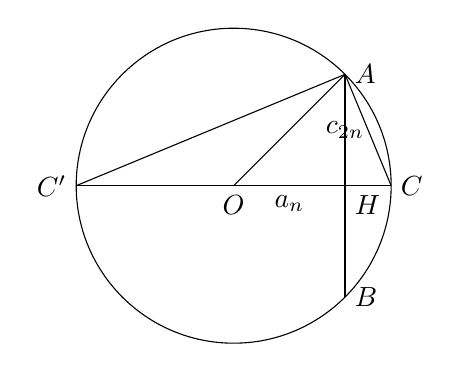
\begin{tikzpicture}
		\draw (0,0) -- (2,0) ;
		\draw (0,0) -- (-2,0) ;
		\draw (0,0) circle (2) ;
	
		\draw (45:2) node[right]{$A$} ;
		\draw (-45:2) node[right]{$B$} ;
		\draw ({sqrt(2)},0) node[below right]{$H$} ;

		\draw (0,0) -- (45:2) ;
		\draw (-2,0) -- (45:2) ;
		\draw (2,0) -- (45:2) ;
		\draw (45:2) -- (-45:2) node[near start] {$c_{2n}$} ;
		\draw (0,0) -- ({sqrt(2)},0) node[midway, below] {$a_{n}$} ;
	
		\draw (0,0) node[below]{$O$} ;
		\draw (2,0) node[right]{$C$} ;
		\draw (-2,0) node[left]{$C'$} ;
	\end{tikzpicture}
	\end{figure}

Dans le triangle rectangle $ACC'$ : 

\begin{align*}
AC^2 &= CC'.CH = CC' (OC - OH) \\
\Leftrightarrow  c_{2n}^2 &= 2R -(R-a_n)
\end{align*}


Or
\begin{align*}
OH &= \sqrt{OA²-AH²} \\
\Leftrightarrow  a_n &= \sqrt{R²-\frac{c_n^2}{4}}
\end{align*}

Donc
$$ c_{2n}^2 = R (2R-\sqrt{4R^2 - c_n^2}) $$
Comme $ c_n = \frac{p_n}{n} $, on obtient :
$$ \frac{p_{2n}^2}{4n^2}=R(2R-\sqrt{4R^2-\frac{p^2}{n^2}}) $$
Soit pour $2R=1$
$$ \boxed{ p_{2n}^2 = 2n (n - \sqrt{n^2-p_n^2}) } $$

En partant d'un carré inscrit $(n=4)$, nous avons $c_4=\frac{\sqrt{2}}{2}$ et donc 
nous pouvons calculer les valeurs de $p_8, p_{16}, p_{32}, \dots$

\subsubsection{Calcul de $p'_n$ en fonction de $p_n$}
Les polygones inscrits et cirsconscrits étant deux polygones semblables, nous avons :
\begin{align*}
\frac{p'_n}{p_n} &= \frac{R}{a_n} \\
\Leftrightarrow  p'_n &= p_n . \frac{R}{a_n} \\
\Leftrightarrow  p'_n &= p_n . \frac{2R}{\sqrt{4R^2 - c_n^2}} \\
\Leftrightarrow  p'_n &= \frac{2nRp_n}{\sqrt{4n^2 R^2 - p_n^2}} 
\end{align*}

Soit pour $2R=1$
$$ \boxed{ p'_n = \frac{np_n}{\sqrt{n^2-p_n^2}} } $$

\begin{tikzpicture}

	\tikzmath{\n = 4; 
			  \p4 = {2*sqrt(2)};
			  \q4 = {\n * \p4 / sqrt(\n^2 - \p4^2)} ;
			  \p8 = {sqrt(2*\n *(\n - sqrt(\n^2 - \p4^2)))} ;
			  \n = 8;
			  \q8 = {\n * \p8 / sqrt(\n^2 - \p8^2)} ;
			  \p16 = {sqrt(2*\n *(\n - sqrt(\n^2 - \p8^2)))} ;
			  \n = 16;
			  \q16 = {\n * \p16 / sqrt(\n^2 - \p16^2)} ;
			  \p32 = {sqrt(2*\n *(\n - sqrt(\n^2 - \p16^2)))} ;
			  \n = 32;
			  \q32 = {\n * \p32 / sqrt(\n^2 - \p32^2)} ;
			  \p64 = {sqrt(2*\n *(\n - sqrt(\n^2 - \p32^2)))} ;
			  \n = 64;
			  \q64 = {\n * \p64 / sqrt(\n^2 - \p64^2)} ;
		%	  \p128 = {sqrt(2*\n *(\n - sqrt(\n^2 - \p64^2)))} ;
		%	  \n = 128;
		%	  \q128 = {\n * \p128 / sqrt(\n^2 - \p128^2)} ;
	        }
	\node[draw,text width=15cm] at(0,0){Les valeurs approchées de $\pi$ par défaut, et par excès en fonction
	du nombre $n$ de côtés :\\
	 $ n=4 \rightarrow \p4 < \pi < \q4 $ \\
	 $ n=8 \rightarrow \p8 < \pi < \q8 $  \\
	 $ n=16 \rightarrow \p16 < \pi < \q16 $ \\
	 $ n=32 \rightarrow \p32 < \pi < \q32 $  \\
	 $ n=64 \rightarrow \p64 < \pi < \q64 $ \\
	% $ n=128 \rightarrow \p128 < \q128 $ \\
	 	 }  ;
\end{tikzpicture}


\vspace{1cm}
Depuis la formule $  p_{2n}^2 = 2n (n - \sqrt{n^2-p_n^2})  $ et sachant que $p_n = n.c_n$, 
nous pouvons en déduire :
$$ c_{2n} = \sqrt{2-\sqrt{4-c_n^2}} $$

Pour un carré de rayon $1$, nous avons $c_4=\sqrt{2}$. Ainsi $c_8= \sqrt{2-\sqrt{2}}$

De même, $c_{16}=\sqrt{2-\sqrt{2+\sqrt{2}}} $  et $c_{32}=\sqrt{2-\sqrt{2+\sqrt{2+\sqrt2}}} $

Comme formule générique, nous obtenons ainsi avec $n-1$ racines imbriquées :
$$c_{2^n}=\sqrt{2-\sqrt{2+\sqrt{2+\sqrt{2+\sqrt{2+\dots}}}}}$$ 

Quand $n$ tend vers l'infini, le $2^n$-gone tend vers le cercle. D'où :
$$ 2^n \sqrt{2-\sqrt{2+\sqrt{2+\sqrt{2+\sqrt{2+\dots}}}}} \rightarrow \pi\ quand\ n \rightarrow \infty $$

Nous pourrons nous référer à \cite{wm}


\subsection{La série alternée de Leibniz}
\[ \sum_{n=0}^\infty \frac{(-1)^n}{2n+1} = \frac{1}{1} -\frac{1}{3}+\frac{1}{5}-\frac{1}{7}+\frac{1}{9} - \dots = \frac{\pi}{4}  \]

Nous pouvons coder cette somme infinie en utilisant un type \textit{stream}. 

\begin{Verbatim}
type 'a stream = Cons of 'a * (unit -> 'a stream) ;;
let hd (Cons (h, _)) = h ;;
let tl (Cons (_, tf)) = tf () ;;

let rec sum n s acc =
	if n=0 then acc
	else  sum (n-1) (tl s) (acc +. (hd s)) ;;

let rec take n s =
	if n=0 then []
	else hd s :: take (n-1) (tl s) ;;

let rec from i = Cons ((((-1.) ** i ) /. (2.*. i +. 1.)), fun () -> from (i +. 1.)) ;;
let leibniz = from 0. ;;
\end{Verbatim}


Cette série est belle, mais paresseuse. Elle converge très lentement vers $\frac{\pi}{4}$. 
Prenons les cinq millions premières valeurs de notre stream \verb+leibniz+.
\begin{Verbatim}
# 4. *. sum 5000000 leibniz 0. ;;
- : float = 3.14159245358977968
\end{Verbatim}


\subsection{La loi des grands nombres}
Sur un tirage aléatoire de coordonnées $(x,y)$ avec $x$ et $y$ compris entre $-1$ et $1$,
il y a  $\pi$ chances sur 4 que le tirage tombe dans le cercle de rayon 1.
\begin{center}
\vspace{0.5cm}
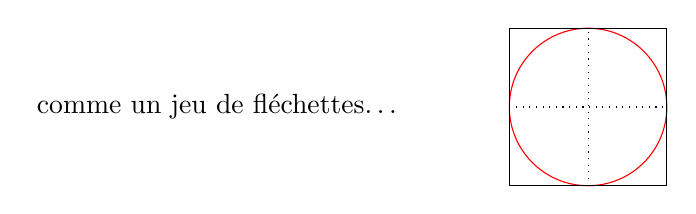
\begin{tikzpicture}
	\draw [dotted] (-1,0) -- (1,0) ;
	\draw [dotted] (0,-1) -- (0,1) ;
	\draw [red] (0,0) circle (1) ;
	\draw (-1,-1) -- (-1,1) -- (1, 1) -- (1,-1) --cycle;
	\node[text width=6cm] at(-4,0){comme un jeu de fléchettes\dots};
\end{tikzpicture}
\end{center} 

Le résultat des tirages est stocké sur notre liste "infinie". Nous effectuons cinq millions de tirages qui nous
permettent d'obtenir une valeur approchée de $\pi$  avec les deux premières décimales exactes.
\begin{Verbatim}
let gen() = 
let x = if Random.bool () then Random.float 1. else (-. Random.float 1.) in
let y = if Random.bool () then Random.float 1. else (-. Random.float 1.) in
if (x ** 2. +. y ** 2. <= 1.) then 1.0 else 0.0 ;;

let rec from i = Cons (gen(), fun () -> from (i + 1)) ;;

let rec sum n s acc =
if n=0 then acc
else  sum (n-1) (tl s) (acc +. (hd s)) ;;
  
4. *. (sum 5000000  tirage 0. /. 5000000.) ;;
- : float = 3.142153
\end{Verbatim}

\subsection{Le produit de Wallis}
Pour introduire le produit infini de Wallis, nous partons du fait que tout polynome
de degré $n$ s'écrivant $f(x) = a_n x^n + a_{n-1} x^{n-1}+ \dots + a_1 x + a_0$ peut se décomposer en :
$$ f(x) = a_n(x-x_1)(x-x_2)\dots(x-x_n)$$
Et en factorisant ce produit par $x_1.x_2\dots x_n$, nous pouvons écrire :
$$ f(x) = C (1-\frac{x}{x_1})(1-\frac{x}{x_2})\dots(1-\frac{x}{x_n}) $$ 
$C$ est ici une constante égale à $a_0$, que nous avons calculé en posant $x=0$.

Euler aurait démontré que cette décomposition vraie pour les polynomes l'est également pour la fonction $\sin(x)$, et plus
particulièrement $\sin(\pi x)$. Nous avons $\sin(\pi\ n)=0\ \forall n \in \mathbb{Z}$
$$\sin (\pi x) = \pi x (1-\frac{x^2}{1^2})(1-\frac{x^2}{2^2})(1-\frac{x^2}{3^2})(1-\frac{x^2}{4^2})\dots $$
Et donc pour $x=\frac{1}{2}$, nous avons :
$$\sin (\frac{\pi}{2}) = 1 = \frac{\pi}{2} (1-\frac{1}{2^2.1^2}) (1-\frac{1}{2^2.3^2}) (1-\frac{1}{2^2.4^2}) \dots $$
Si nous écrivons 
$$1-\frac{1}{2^2.n^2} = \frac{(2n-1)(2n+1)}{2n.2n} $$
Nous obtenons le produit de Wallis :

\[ \frac{\pi}{2} = ( \frac{2}{1}.\frac{2}{3} ) . (\frac{4}{2}.\frac{4}{5} ).(\frac{6}{5}.\frac{6}{7} ).(\frac{8}{7}.\frac{8}{9} ) . ...  =  \prod_{n=1}^\infty \frac{2n.2n}{(2n-1).(2n+1)} = \prod_{n=1}^\infty \frac{4n^2}{4n^2-1}\]
\vspace{0.3cm}	
\begin{Verbatim}
let rec from i = Cons ((4. *. i**2. ) /. (4. *. i**2. -. 1.), fun () -> from (i +. 1.)) ;;
let wallis = from 1. ;;

let rec mult n s acc =
	if n=0 then acc
	else  mult (n-1) (tl s) (acc *. (hd s)) ;;
\end{Verbatim}
Le produit converge ici rapidement vers $\pi /2$. Nous multiplions les cinquantes premiers millions 
de notre liste infinie \verb+wallis+.
\begin{Verbatim}
utop # 
2. *. mult 5000000 wallis 1. ;;
- : float = 3.14159249652297845
\end{Verbatim}

\subsection{L'intégrale $\int_0^1 \frac{1}{1+x^2} dx$}
\begin{tikzpicture}
	\draw[->] (-0.5, 0) -- (1.5, 0) node[right] {$x$};
	\draw[->] (0, -0.5) -- (0, 1.5) node[above] {$y$};
	\draw node[below left]{$0$} ;
	\draw (1,0) node[below]{$1$}  ;
	\draw[domain=-0.5:1.5, smooth, variable=\x, blue] plot (\x, {1 /( 1 + \x^2});
	\fill [pattern=north east lines]
	   (0,0)
	  -- (1,0)
	  -- (1,0.5)
	  -- plot [domain=0:1]  (\x, {1 /( 1 + \x^2)})
	  -- (0,1) 
	  -- cycle;
	\node[text width=7cm] at(6,1){$$\int_0^1 \frac{1}{1+x^2} dx  = \lim_{n\rightarrow \infty}  \frac{1}{n} \sum_{i=0}^n \frac{1}{1+(\frac{i}{n})^2} = \frac{\pi}{4}$$};
\end{tikzpicture}
 
\begin{Verbatim}
let f x = 1. /. (1. +. x**2.)

let rec somme n i acc =
  if i > n then (1./. n) *. acc 
  else somme n (i +. 1.)  (acc +. (f (i /. n))) ;;

utop # 
 4. *. somme 900000000. 0. 0. ;;
 - : float = 3.14159265692298773
\end{Verbatim}

\section{Poésies}
\begin{verse}
	Un soir t'en souvient-il ? Nous voguions en silence ; \\
	On n’entendait au loin, sur l’onde et sous les cieux,  \\
	Que le bruit des rameurs qui frappaient en cadence     \\
	Tes flots harmonieux. \\
\end{verse}

\begin{verse}
	Les feuilles mortes se ramassent à la pelle \\
	Tu vois, je n'ai pas oublié... \\
	Les feuilles mortes se ramassent à la pelle, \\
	Les souvenirs et les regrets aussi \\
\end{verse}

\begin{verse}
	Agneau de Dieu, qui sauves les hommes, \\
	Agneau de Dieu, qui nous comptes et nous nommes, \\
	Agneau de Dieu, vois, prends pitié de ce que nous sommes. \\
\end{verse}

\begin{verse}
	Demain, dès l'aube, à l'heure où blanchit la campagne, \\
	Je partirai. Vois-tu, je sais que tu m'attends. \\
	J'irai par la forêt, j'irai par la montagne. \\
	Je ne puis demeurer loin de toi plus longtemps. \\
\end{verse}

\section{Lectures}
Call me Ismaël. \cite{moby}

Some years ago - never mind how long precisely - having little or no money in my purse, 
and nothing particular to interest me on shore,
I thought I would sail about a little and see the watery part of the world. 
\section{Les fractions continues}

$$
\frac{32}{7} = 4+\cfrac{1}{1+\cfrac{1}{1+\cfrac{1}{3}}}
$$


\begin{Verbatim}
let cont a b =
  let rec aux acc a b =
    if a mod b = 0 then
      a::acc
    else  aux ((a / b)::acc) b (a mod b)
  in rev (aux [] a b) ;;

(* 
[4;1;1:3]
4+\cfrac{1}{1+\cfrac{1}{1+\cfrac{1}{3}}}
*)

let rec print = function
  | [] -> ""
  | h::[] -> string_of_int h 
  | h::t ->  string_of_int(h) ^ " + \\cfrac{1}{" ^ print t ^ "}" ;;
\end{Verbatim}

\section{L'irrationalité de $\sqrt{2}$}
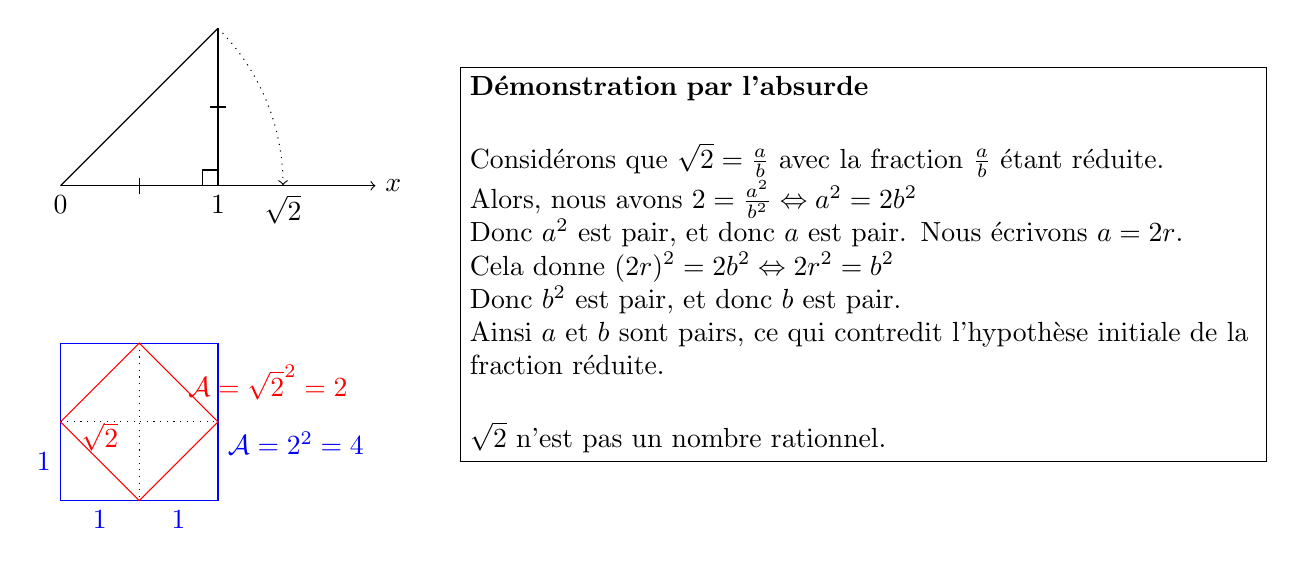
\begin{tikzpicture}[scale=2]
	\draw[->] (0, 0) -- (2, 0) node[right] {$x$};
	\draw (0, 0) -- (1, 1)  ;
	\draw (0,0) node[below] {$0$} ;
	\draw (1,0) node [below]  {$1$} ;
	\draw (0, 0) -- (1, 0)  ;
	\draw (1, 1) -- (1, 0)  ;
	\draw [dotted, ->] (1,1) arc (45:0:1.41) node[below] {$\sqrt{2}$} ;
	\draw (0.5,-0.05) -- (0.5,0.05) ;
	\draw (0.95,0.5) -- (1.05,0.5)  ;
	\draw (0.9,0) -- (0.9,0.1) --(0.9,0.1) -- (1,0.1) ;
	

	\draw [blue]  (0,-1) -- (1,-1) -- node[below right] {$\mathcal{A} = 2^2 = 4$ } (1,-2) -- 
	      node[below] {$1$} (0.5, -2) -- node[below] {$1$} (0,-2) -- node[left] {$1$} (0, -1.5) -- cycle ;
	\draw [red] (0.5,-1) -- node[right] {$\mathcal{A} = \sqrt{2}^2 = 2$ } (1,-1.5) -- (0.5,-2) -- 
	       node[above ] {$\sqrt{2}$} (0.,-1.5) -- cycle ;

	\draw [dotted] (0,-1.5) -- (1,-1.5) ;
	\draw [dotted] (0.5,-1) -- (0.5,-2) ;

	\node[draw,text width=10cm] at(5.1,-0.5){\textbf{Démonstration par l'absurde}\\
      \vspace{0.5cm}
	
	Considérons que $\sqrt{2}=\frac{a}{b}$ avec la fraction $\frac{a}{b}$ étant réduite. \\
    Alors, nous avons $2 = \frac{a^2}{b^2} \Leftrightarrow a^2 = 2b^2 $ \\
    Donc $a^2$ est pair, et donc $a$ est pair. Nous écrivons $a=2r$. \\
    Cela donne $(2r)^2 = 2b^2 \Leftrightarrow 2r^2 = b^2 $ \\
    Donc $b^2$ est pair, et donc $b$ est pair. \\
    Ainsi $a$ et $b$ sont pairs, ce qui contredit l'hypothèse initiale de la fraction réduite. \\
	
	\vspace{0.5cm}
    \imp $\sqrt{2}$ n'est pas un nombre rationnel.		  
	};
\end{tikzpicture}

\section{Démonstration non constructive}
Démontrons qu'il existe deux irrationnels $a$ et $b$ tels que $a^b$ soit rationnel.

Considérons $\sqrt{3}^{\sqrt{2}}$ 

Si  $\sqrt{3}^{\sqrt{2}} \in \mathbb{Q}$ alors on pose $a = \sqrt{3}$ et $b= \sqrt{2}$

Sinon, on pose $a = \sqrt{3}^{\sqrt{2}}$ et $b=\sqrt{2}$, 
de sorte que $ {(\sqrt{3}^{\sqrt{2}})}^{\sqrt{2}} = 3 \in \mathbb{Q} $


Mais laquelle des deux est la solution ?
Faut-il abandonner le principe du \textit{tiers-exlus} de nos démonstrations
mathématiques ?
\section{Le tout est-il plus grand que chacune de ses parties ?}
Galilée remontait le paradoxe suivant sur les nombres entiers : Chaque entier peut être mappé 
un à un avec son carré. Pourtant l'ensemble de nombres carrés est intuitivement un sous-ensemble
des nombres entiers.


\begin{tabular}{cccccccccccc}
1 &2 &3 &4  &5  &6  &7  &8  &9  &10  &11  & \ldots \\  
1 &4 &9 &16 &25 &36 &49 &64 &81 &100 &121 & \ldots 
\end{tabular}

\section{L'hyperbole $xy=1$}
\begin{tikzpicture}
	\draw[->] (-3, 0) -- (3, 0) node[right] {$x$};
	\draw[->] (0, -3) -- (0, 3) node[above] {$y$};
	\draw[domain=0.3:3, smooth, variable=\x, blue] plot (\x, {1 / \x});
	\draw[domain=-3:-0.3, smooth, variable=\x, blue] plot (\x, {1 / \x});
	\draw[red] (0.5,0) -- (0.5,2) ;
	\draw[red] (0,2) -- (0.5,2) node [right] {L'aire du rectangle rouge est égale à 1}  ;
\end{tikzpicture}

\section{L'exponentielle}
\begin{align*}
e^x &= 1 + x + \frac{x^2}{2} + \frac{x^3}{6} + \frac{x^4}{24} + \dots + \frac{x^n}{n!} + \dots \\
    &= \sum_{k=0}^{\infty} \frac{x^k}{k!} \\
\end{align*}
Nous avons ainsi : $e= 1+1+\frac{1}{2}+\frac{1}{6} +\frac{1}{24}+ \dots + + \frac{1}{n!} + \dots $ \\
Et également $e = \lim_{n \rightarrow \infty} (\frac{1}{1+n})^n $

\section{Les fonctions $\sin \frac{1}{x}$ et $x . \sin \frac{1}{x}$ }
\begin{center}
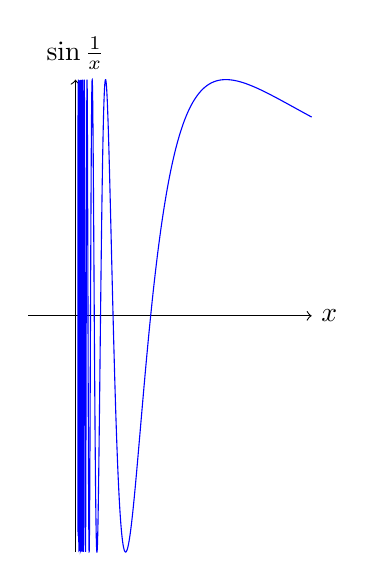
\begin{tikzpicture}[scale =3]
	\draw[->] (-0.2, 0) -- (1, 0) node[right] {$x$};
	\draw[->] (0, -1) -- (0, 1) node[above] {$\sin \frac{1}{x}$};
	\draw[domain=0.01:1, samples=5000,  smooth, variable=\x, blue] plot (\x, {sin((1/\x)r)});
\end{tikzpicture}
\hspace{1cm}
\begin{tikzpicture}[scale =3]
	\draw[->] (-0.2, 0) -- (1, 0) node[right] {$x$};
	\draw[->] (0, -1) -- (0, 1) node[above] {$x . \sin \frac{1}{x}$};
	\draw[domain=0.01:1, samples=5000,  smooth, variable=\x, blue] plot (\x, {\x * sin((1/\x)r)});
    \draw[domain=0.01:1,   smooth, variable=\x, red] plot (\x, {\x});
    \draw[domain=0.01:1,   smooth, variable=\x, red] plot (\x, {-\x});
\end{tikzpicture}
\end{center}
%%%%%%%%%%%%%%%%%%%%%%%%

\section{Srivanasa Ramanujan}
Le mathématicien indien aurait  découvert la très belle formule 
$$ 3 = \sqrt{1+2\sqrt{1+3\sqrt{1+4\sqrt{1+\ldots}}}} $$
Posons $f(n) = n(n+2)$, et sachant que $n(n+2) = n \sqrt{1+(n+1)(n+3)}$, nous avons :

\begin{align*}
	f(n) &= n\sqrt{1+f(n+1)} \\
	 	 &= n\sqrt{1+(n+1)\sqrt{1+f(n+2)}} \\
	 	 &= n\sqrt{1+(n+1)\sqrt{1+(n+2)\sqrt{1+f(n+3)}}}
\end{align*}

\begin{Verbatim}
let rec f n i =
 if i = 0 then 1.
 else n *. sqrt(1. +. (f (n +. 1.) (i-1)))

utop # f 1. 10 ;;
- : float = 2.99480026926620502
\end{Verbatim}

Nous pouvons définir la fonction d'affichage \verb+f_latex+ comme ci-dessous:
\begin{Verbatim}
let rec f_latex n i =
  if i = 0 then "\\ldots"  
  else (string_of_int n)^ "\\sqrt{1 + " ^ (f_latex (n + 1) (i-1)) ^ "}" ;;

print_string (f_latex 1 10) ;;	
\end{Verbatim}
$$3 = 1\sqrt{1 + 2\sqrt{1 + 3\sqrt{1 + 4\sqrt{1 + 5\sqrt{1 + 6\sqrt{1 + 7\sqrt{1 + 8\sqrt{1 + 9\sqrt{1 + 10\sqrt{1 + \ldots}}}}}}}}}}
$$
\section{Le grec ancien}
\subsection{L'alphabet grec}
\[
\begin{array}{cccccccccccccccccccccccc}
 \alpha & \beta &\gamma &  \delta & \epsilon & \zeta & \eta &\theta & \iota &\kappa &\lambda & \mu & \nu & \xi & o & \pi & \rho & \sigma & \tau & 
 \upsilon & \phi & \chi & \psi & \omega \\
 A & B & \Gamma & \Delta & E & Z & H & \Theta & I & K & \Lambda & M & N  &\Xi & O & \Pi & R & \Sigma & T & \Upsilon & \Phi & X & \Psi & \Omega
 \end{array}
 \]

\subsection{Les mathématiques grecques}
\begin{tabular}{c | c}
 j'apprends & \textgreek{mathano} \\
 l'étude, la leçon & \textgreek{to mathema} \\
 l'étude par excellence & \textgreek{ta mathematija} \\
\end{tabular}

\subsection{Extraits du nouveau testament}
 \begin{center}

\begin{tikzpicture}
  \draw [line width=0.7mm, smooth, tension=1] plot coordinates{(0,0) (1,-0.5) (2.1, 0) (2.5, 0.55)} ;
  \draw [line width=0.7mm, smooth, tension=1] plot coordinates{(0,0) (1,0.5) (2.1, 0) (2.5,-0.55)} ;
  \draw node at (1.1,0) {\textgreek{IQJUS}} ;
\end{tikzpicture} 
\\
\textgreek{Ἰησοῦς  Χριστὸς Θεοῦ Υἱὸς Σωτήρ} 
\end{center}

\vspace{1cm}

 \textgreek{	
Ἐγὼ τὸ Ἄλφα  καὶ τὸ Omega, ὁ  πρῶτος καὶ ὁ ἔσχατος, ἡ ἀρχὴ καὶ τὸ τέλος

Ἄλλην παραβολὴν παρέθηκεν αὐτοῖς, λέγων, Ὁμοία ἐστὶν ἡ βασιλεία τῶν οὐρανῶν
κόκκῳ σινάπεως, ὃν λαβὼν ἄνθρωπος ἔσπειρεν ἐν τῷ ἀγρῷ αὐτοῦ:
ὃ μικρότερον μέν ἐστιν πάντων τῶν σπερμάτων: ὅταν δὲ αὐξηθῇ,
μεῖζον τῶν λαχάνων ἐστίν, καὶ γίνεται δένδρον, ὥστε ἐλθεῖν τὰ πετεινὰ τοῦ οὐρανοῦ 
καὶ κατασκηνοῦν ἐν τοῖς κλάδοις αὐτοῦ.

Eirene umin !
}